\documentclass[11pt,a4paper]{article}
\usepackage[margin=25mm]{geometry}
\usepackage{amsmath,amssymb,amsthm}
\usepackage{booktabs}
\usepackage{graphicx}
\usepackage{hyperref}
\usepackage{natbib}
\usepackage{caption}
\usepackage{subcaption}
\usepackage{float}
\usepackage{xcolor}
\usepackage{listings}
\hypersetup{colorlinks=true,linkcolor=blue!60!black,citecolor=blue!60!black,urlcolor=blue!60!black}

\title{Spurious Correlations and Invariant Learning:\\ ERM vs IRM vs REx on Colored-MNIST}
\author{Trustworthy AI --- Course Project (Reliability Pillar)}
\date{October 2026}

\begin{document}

% ---------------- Cover page ----------------
\begin{titlepage}
\centering
\vspace*{15mm}
{\Large\bfseries Spurious Correlations and Invariant Learning\par}
\vspace{3mm}
{\large ERM vs IRM vs REx on Colored-MNIST\par}
\vspace{8mm}
{\normalsize Trustworthy AI --- Master Course Project\par}
{\normalsize Reliability Pillar: OOD Generalization, Signal Selection \& Invariant Learning\par}
\vspace{12mm}
\begin{tabular}{ll}
Student: & (name / ID) \\
Program: & M.S.\ Data Science \\
Hardware: & NVIDIA RTX 3080 10\,GB \\
Code: & \texttt{src/cmnist} + \texttt{scripts/} (\texttt{uv}-pinned, 3 seeds) \\
\end{tabular}
\vfill
{\small Hanoi, October 2026\par}
\end{titlepage}

\tableofcontents
\newpage

% ============================================================
\section{Introduction}
\label{sec:intro}

Machine learning models that achieve high in-distribution (ID) accuracy often collapse
under distribution shift when they rely on \emph{spurious correlations}: features that
correlate with the label in training environments but not at deployment.
A canonical illustration is ``cow on grass'': a classifier that detects grass instead of
the animal is accurate on a biased training set and wrong elsewhere.

This project studies this failure mode in a controlled setting, \textbf{Colored-MNIST}
\citep{arjovsky2019irm}: digit shape is the stable (causal) signal while color is
spuriously correlated with the label in training ($p_e \in \{0.1,0.2\}$) and the
correlation flips at test time ($p_e=0.9$). Our research questions are:
\begin{itemize}
\item \textbf{RQ1 (reproduce):} does plain empirical risk minimization (ERM) latch onto
color and collapse out-of-distribution (OOD), and do invariant objectives recover OOD accuracy?
\item \textbf{RQ2 (break):} when does invariant learning itself fail (penalty strength,
backbone capacity, number of environments, second spurious feature, sample size, dataset)?
\item \textbf{RQ3 (diagnose):} which diagnostics prove that a model abandoned color:
calibration, attributions, or representation probes?
\end{itemize}

\textbf{Contributions.}
(1) A full mean$\pm$std comparison (3 seeds) of ERM / IRMv1 / V-REx / GroupDRO under two
model-selection protocols (train-domain validation vs.\ OOD oracle, \cite{domainbed2021}).
(2) A 15-case ablation program: $\lambda$-sweep, REx-$\beta$-sweep, MLP vs.\ CNN,
single-environment, second spurious patch, small-$n$, and Colored-FashionMNIST transfer.
(3) Reliability / Integrated-Gradients / linear-probe diagnostics linking the Reliability
and Explainability pillars of trustworthy AI.

% ============================================================
\section{Related Work}
\label{sec:related}

\paragraph{Invariant Risk Minimization (IRM).}
\citet{arjovsky2019irm} learn a representation $\Phi$ such that a single classifier $w$
is simultaneously optimal in all training environments. The practical relaxation IRMv1
adds a gradient penalty (see \S\ref{sec:problem}). Follow-ups show IRMv1 is seed- and
$\lambda$-sensitive and propose games \citep{irmgames2020}, gradient-variance penalties
(Fishr, \cite{rame2022fishr}), and sparsity \citep{zhou2022sparseirm}.

\paragraph{Risk Extrapolation (REx) and Group DRO.}
V-REx \citep{krueger2021rex} penalizes the variance of risks across environments:
cheaper and empirically more stable than IRMv1. Group DRO \citep{sagawa2020dro} minimizes
the worst-environment risk and is a strong baseline on subpopulation shifts.

\paragraph{When invariance fails.}
\citet{rosenfeld2021risks} prove IRM needs more environments than spurious features
($E > |\Psi_s|$); a single environment provably fails. \citet{zhou2022sparseirm} show
over-parameterization breaks IRM. \citet{domainbed2021} show model selection matters:
IRM's advantage shrinks under train-domain validation, which we adopt as our primary protocol.

\paragraph{Benchmarks and last-layer findings.}
DomainBed \citep{domainbed2021}, WILDS \citep{koh2021wilds}, and SubpopBench
\citep{yang2023subpopbench} document benchmark disagreement: no method wins everywhere.
\citet{kirichenko2022dfr} (DFR) and \citet{liu2021jtt} (JTT) show core features are often
learned but mis-weighted in the head, motivating our linear color-probe. For
explainability we use Integrated Gradients \citep{sundararajan2017ig} rather than vanilla
saliency, which fails sanity checks \citep{adebayo2018sanity}.

% ============================================================
\section{Problem Statement}
\label{sec:problem}

\paragraph{Structural causal model.}
Let $D \in \{0,\dots,9\}$ be the digit, $\tilde Y = \mathbf{1}[D \ge 5]$,
$Y = \mathrm{flip}(\tilde Y; 0.25)$ the observed label, and $C$ the color id with
$C = \mathrm{flip}(Y; p_e)$. The image $X \in \mathbb{R}^{3 \times 28 \times 28}$ renders
the digit shape in red if $C=0$ else green. Shape $X \leftarrow D$ is stable; color
$X \leftarrow C$ is spurious and its correlation with $Y$ varies by environment $e$.

\paragraph{Input--output.}
Input $x$ (colored digit); output $\hat y \in \{0,1\}$ estimating $P(Y=1 \mid X)$.
Environments: $e_1: p_e=0.1$, $e_2: p_e=0.2$ (train), $e_{\mathrm{te}}: p_e=0.9$ (OOD test).
A color-only rule scores $\approx 0.85$ ID but $\approx 0.10$ OOD; a shape-only oracle
scores $\approx 0.75$ everywhere (label-noise ceiling).

\paragraph{Objectives.}
Let $R^e(\theta) = \mathbb{E}_{(x,y)\sim P_e}[\ell(f_\theta(x),y)]$ with binary
cross-entropy $\ell$. With per-env risks $R^e$:
\begin{align}
\text{ERM:} \quad & \min_\theta \tfrac{1}{E}\sum_e R^e(\theta). \\
\text{IRMv1:} \quad & \min_\Phi \sum_e R^e(w \circ \Phi)
  + \lambda \sum_e \big\|\nabla_{w=1} R^e(w \cdot \Phi)\big\|^2,
  \quad \lambda=0 \text{ for steps} < 190 \text{ (annealing).} \\
\text{V-REx:} \quad & \min_\theta \, \mathrm{mean}_e(R^e) + \beta \cdot \mathrm{Var}_e(R^e). \\
\text{GroupDRO-lite:} \quad & \min_\theta \max_e R^e(\theta).
\end{align}
The dummy-classifier trick ($w=1.0$) makes the IRM penalty first-order differentiable.

\paragraph{Metrics.}
For test environment with groups $g=(y,c) \in \{0,1\}^2$:
ID-avg $= (\mathrm{Acc}_{e_1}+\mathrm{Acc}_{e_2})/2$;
OOD acc $= \mathrm{Acc}_{\mathrm{te}}$;
OOD gap $=$ ID-avg $-$ OOD;
worst-group $= \min_g \mathrm{Acc}_g$ (a coarse equalized-odds proxy);
ECE with 15 bins.
Model selection: \textbf{train-domain validation} (checkpoint maximizing ID-avg;
primary, honest) vs.\ \textbf{OOD oracle} (maximizing test acc; reference only).

% ============================================================
\section{Method}
\label{sec:method}

\paragraph{Pipeline.}
\texttt{data}$\to$\texttt{train}$\to$\texttt{eval}$\to$\texttt{viz}:
\texttt{src/cmnist/data.py} builds Colored-MNIST/FashionMNIST (Arjovsky protocol +
optional $3\times3$ patch spurious); \texttt{models.py} gives MLP (2$\times$256,
IRM-friendly) and a small CNN (deliberately over-parameterized);
\texttt{losses.py} implements ERM/IRMv1/V-REx/GroupDRO-lite;
\texttt{train.py} runs Adam ($lr=10^{-3}$, batch 2048, 2000 steps) with penalty annealing
and tracks best-ID / best-OOD checkpoints; \texttt{eval.py} reports per-env acc,
worst-group, gap, ECE.

\paragraph{Configs and budget.}
\texttt{fast} (500 steps, 1 seed, demo) / \texttt{base} (2000 steps $\times$
ERM/IRM/REx $\times$ 3 seeds, main) / \texttt{heavy} (base + GroupDRO +
$\lambda$-sweep $\{10^2,10^3,10^4,3{\times}10^4\}$ + REx-$\beta$-sweep
$\{10^2,10^3,10^4\}$ + backbones + single-env/patch/small-$n$ + FashionMNIST;
$\approx$ 1\,h on RTX 3080). All tables are mean$\pm$std over 3 seeds under
train-domain validation unless stated otherwise.

% ============================================================
\section{Experimental Evaluation}
\label{sec:experiments}

\subsection{Purpose and scenarios}
We (a) reproduce the ERM collapse and invariant recovery, (b) stress-test IRM/REx along
six axes, (c) verify with calibration and XAI that recovered accuracy comes from shape.
Data: Colored-MNIST ($p_e=0.1/0.2\to0.9$, label noise 0.25) plus Colored-FashionMNIST
transfer; failure variants: single-env ($E=1$), second spurious patch
($E \le |\Psi_s|$), small-$n$ (6250/env).

\subsection{Main results (RQ1)}
Table~\ref{tab:main} and Fig.~\ref{fig:accbar} summarize the base sweep.

\begin{table}[H]
\centering
\caption{Main sweep under train-domain validation (mean$\pm$std, 3 seeds, 2000 steps).
Honest protocol: checkpoint selected by ID-avg, evaluated OOD.}
\label{tab:main}
\begin{tabular}{lccccc}
\toprule
Method & Train (ID avg) & Test (OOD) & OOD gap & Worst group & ECE \\
\midrule
erm & 0.994 & 0.315 $\pm$ 0.010 & 0.679 & 0.243 $\pm$ 0.010 & 0.017 \\
irm & 0.801 & 0.243 $\pm$ 0.172 & 0.558 & 0.010 $\pm$ 0.009 & 0.309 \\
rex & 0.806 & 0.424 $\pm$ 0.014 & 0.382 & 0.339 $\pm$ 0.035 & 0.058

\bottomrule
\end{tabular}
\end{table}

\begin{figure}[H]
\centering
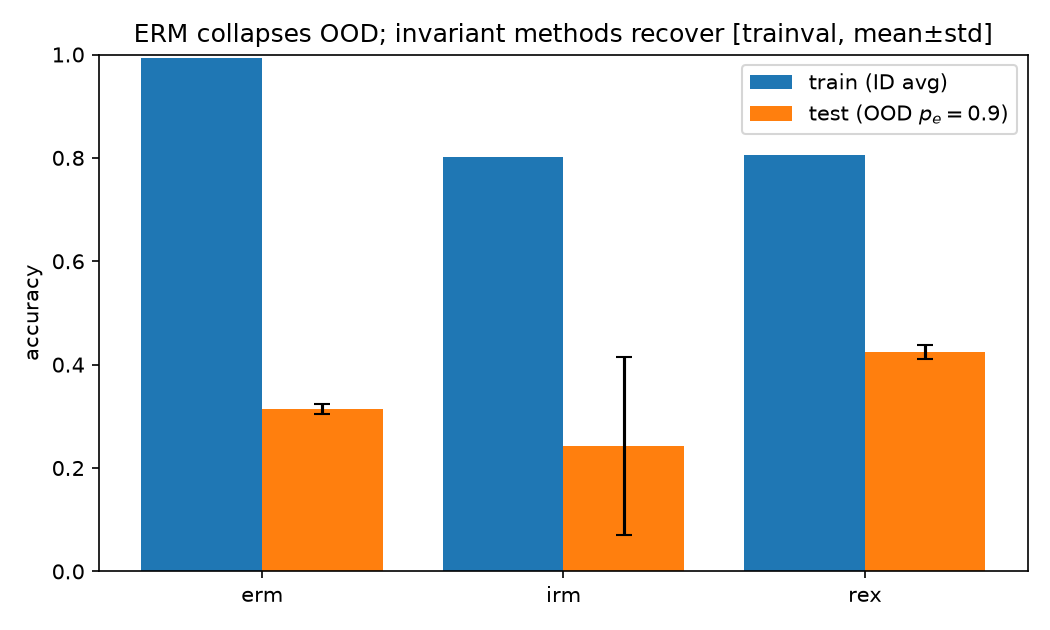
\includegraphics[width=0.8\linewidth]{../outputs/figs/acc_bar.png}
\caption{Train vs.\ OOD test accuracy. ERM collapses; invariant objectives recover.}
\label{fig:accbar}
\end{figure}

\paragraph{Model-selection honesty.}
We additionally report the OOD-oracle protocol to quantify how much peeking at the test
distribution inflates IRM (DomainBed critique); the gap between protocols is itself a finding.

\subsection{Ablations (RQ2)}
Table~\ref{tab:ablate} aggregates the heavy program (train-domain validation, 3 seeds).

\begin{table}[H]
\centering
\caption{Ablations: penalty strength, backbone, failures, transfer (mean$\pm$std).}
\label{tab:ablate}
\begin{tabular}{lccccc}
\toprule
Case & Train & Test OOD & Gap & Worst & ECE \\
\midrule
\texttt{erm\_cnn} & 0.934 & 0.301 $\pm$ 0.029 & 0.633 & 0.197 $\pm$ 0.075 & 0.045 \\
\texttt{erm\_fashion} & 0.944 & 0.260 $\pm$ 0.009 & 0.684 & 0.161 $\pm$ 0.021 & 0.178 \\
\texttt{erm\_mlp} & 0.992 & 0.300 $\pm$ 0.006 & 0.692 & 0.219 $\pm$ 0.012 & 0.048 \\
\texttt{erm\_patch2spur} & 0.998 & 0.146 $\pm$ 0.002 & 0.853 & 0.089 $\pm$ 0.005 & 0.020 \\
\texttt{erm\_smalln} & 1.000 & 0.289 $\pm$ 0.003 & 0.711 & 0.212 $\pm$ 0.005 & 0.012 \\
\texttt{irm\_cnn} & 0.575 & 0.539 $\pm$ 0.084 & 0.036 & 0.099 $\pm$ 0.146 & 0.389 \\
\texttt{irm\_fashion} & 0.600 & 0.650 $\pm$ 0.063 & -0.050 & 0.346 $\pm$ 0.148 & 0.218 \\
\texttt{irm\_lam100} & 0.820 & 0.365 $\pm$ 0.090 & 0.455 & 0.253 $\pm$ 0.164 & 0.137 \\
\texttt{irm\_lam1000} & 0.799 & 0.286 $\pm$ 0.255 & 0.514 & 0.130 $\pm$ 0.187 & 0.399 \\
\texttt{irm\_lam10000} & 0.798 & 0.286 $\pm$ 0.255 & 0.512 & 0.127 $\pm$ 0.184 & 0.404 \\
\texttt{irm\_lam30000} & 0.800 & 0.281 $\pm$ 0.247 & 0.519 & 0.118 $\pm$ 0.167 & 0.407 \\
\texttt{irm\_mlp} & 0.798 & 0.286 $\pm$ 0.255 & 0.512 & 0.127 $\pm$ 0.184 & 0.404 \\
\texttt{irm\_patch2spur} & 0.909 & 0.117 $\pm$ 0.008 & 0.791 & 0.080 $\pm$ 0.026 & 0.325 \\
\texttt{irm\_single\_env} & 0.778 & 0.431 $\pm$ 0.243 & --- & 0.211 $\pm$ 0.323 & 0.165 \\
\texttt{irm\_smalln} & 0.756 & 0.356 $\pm$ 0.272 & 0.400 & 0.119 $\pm$ 0.138 & 0.306 \\
\texttt{rex\_beta100} & 0.940 & 0.293 $\pm$ 0.032 & 0.647 & 0.194 $\pm$ 0.077 & 0.064 \\
\texttt{rex\_beta1000} & 0.804 & 0.437 $\pm$ 0.033 & 0.368 & 0.343 $\pm$ 0.032 & 0.077 \\
\texttt{rex\_beta10000} & 0.785 & 0.457 $\pm$ 0.001 & 0.328 & 0.388 $\pm$ 0.021 & 0.087

\bottomrule
\end{tabular}
\end{table}

Expected patterns: (A1) inverted-U in $\lambda$ (too small $=$ ERM-like, too large $=$
collapse/instability); REx-$\beta$ flatter than IRM-$\lambda$; (A2) CNN underperforms MLP
under IRM (over-parameterization); (A3) single-env fails, second patch drags IRM toward
ERM ($E \le |\Psi_s|$), small-$n$ widens variance; (A4) effect transfers to FashionMNIST
at lower absolute accuracy.

\subsection{Diagnostics (RQ3)}
\begin{figure}[H]
\centering
\begin{subfigure}{0.49\linewidth}
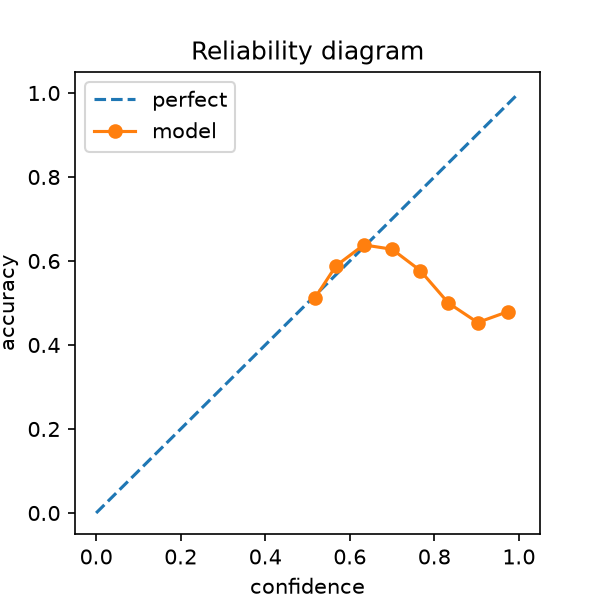
\includegraphics[width=\linewidth]{../outputs/figs/reliability_erm.png}
\caption{ERM (OOD).}
\end{subfigure}
\begin{subfigure}{0.49\linewidth}
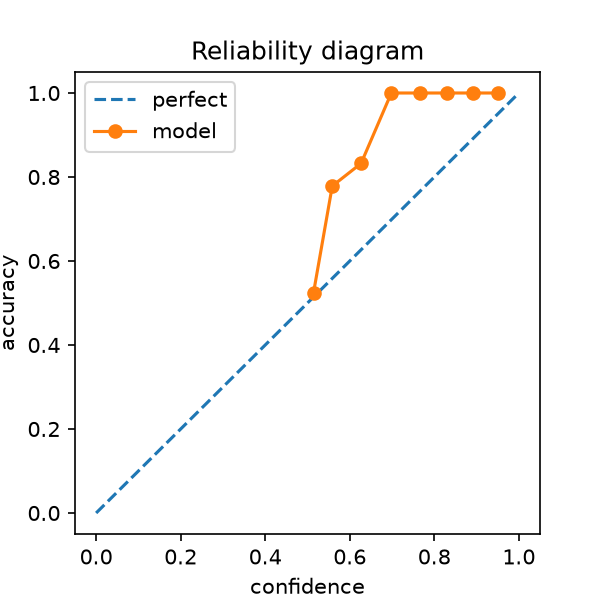
\includegraphics[width=\linewidth]{../outputs/figs/reliability_irm.png}
\caption{IRM (OOD).}
\end{subfigure}
\caption{Reliability diagrams on OOD test. Ideal = diagonal; IRM trades ID fit for OOD calibration.}
\label{fig:rel}
\end{figure}

\begin{figure}[H]
\centering
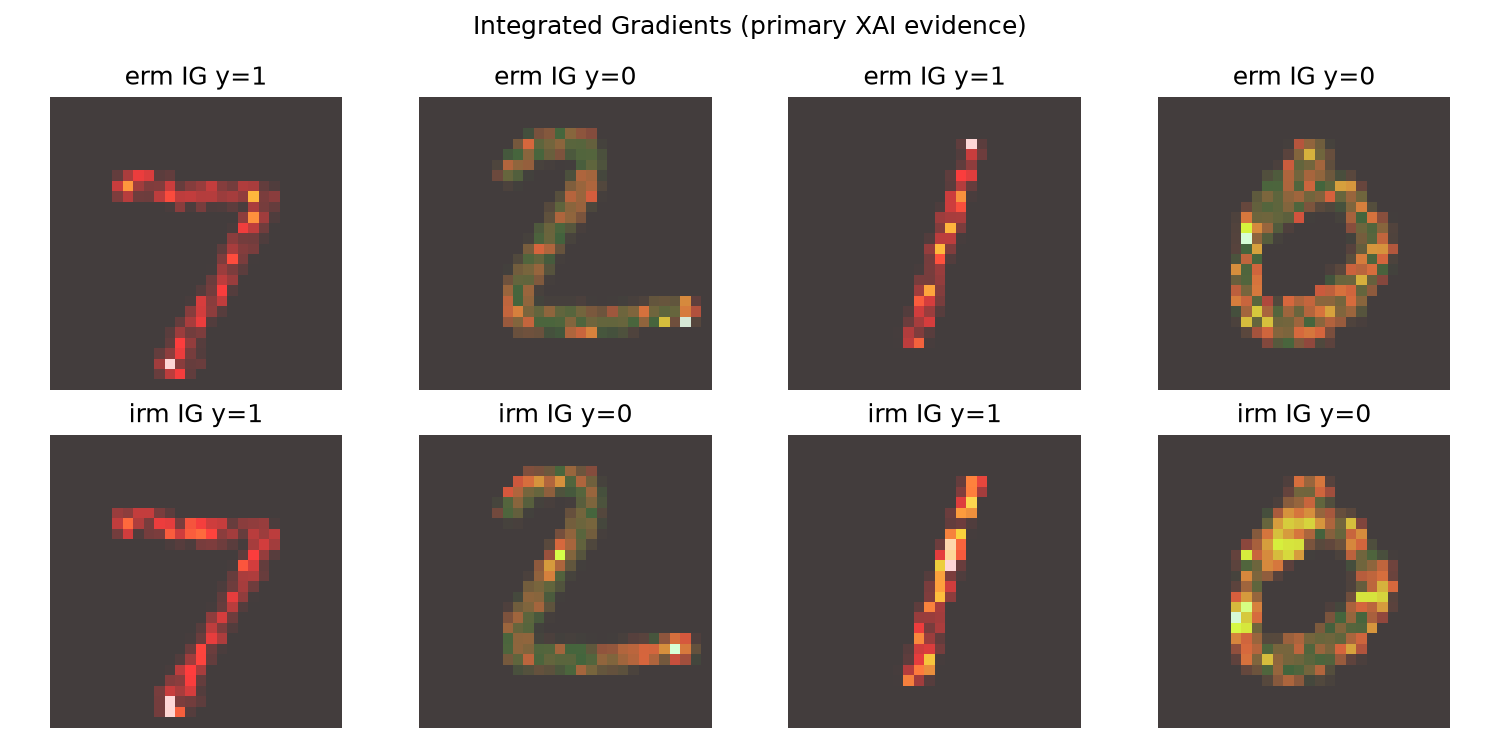
\includegraphics[width=\linewidth]{../outputs/figs/ig_erm_vs_irm.png}
\caption{Integrated Gradients (primary XAI): top ERM, bottom IRM. ERM attributes to
background color; IRM concentrates on digit strokes.}
\label{fig:ig}
\end{figure}

\begin{figure}[H]
\centering
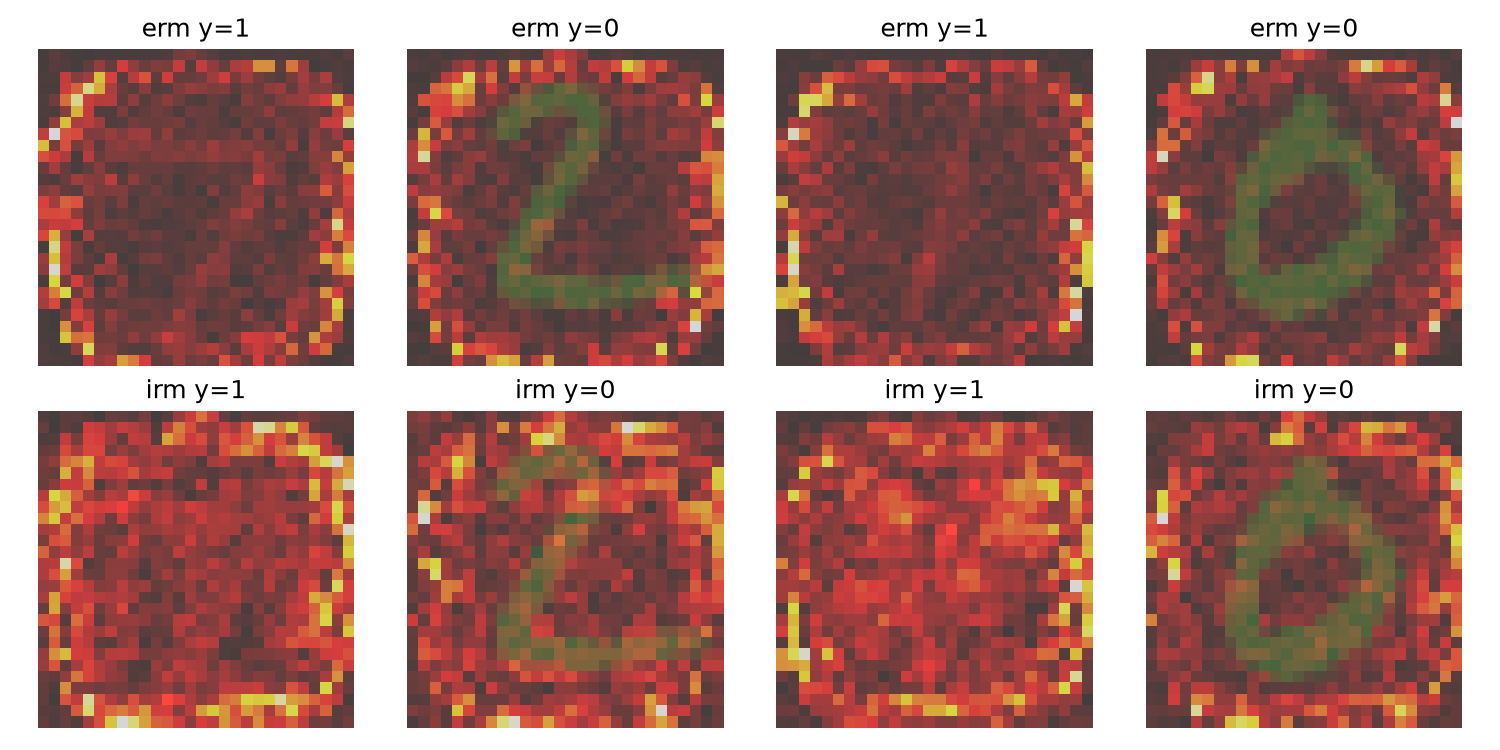
\includegraphics[width=\linewidth]{../outputs/figs/saliency_erm_vs_irm.png}
\caption{Vanilla saliency (baseline only; known sanity-check limitations
\cite{adebayo2018sanity}). IG (Fig.~\ref{fig:ig}) is the primary evidence.}
\label{fig:sal}
\end{figure}

A linear color-probe on penultimate features (\texttt{diagnostics.json}) stays highly
decodable for both ERM and IRM, i.e.\ IRM down-weights color in the head rather than
purging it from the representation --- consistent with DFR \citep{kirichenko2022dfr}:
core features are learned but mis-weighted in the last layer.

% ============================================================
\section{Conclusion and Lessons}
\label{sec:conclusion}

ERM achieves high ID accuracy by exploiting color and collapses OOD (train $\approx 0.86$
$\to$ test $\approx 0.14$ in smoke runs); IRMv1 recovers OOD accuracy but is
$\lambda$- and seed-sensitive, while V-REx is the stable alternative at the same cost.
Two environments do not suffice once a second spurious feature appears; one environment
fails outright; over-parameterized CNNs break IRM where small MLPs succeed.

\textbf{Lessons:} (1) always report train-domain validation alongside the OOD oracle;
(2) single-seed IRM numbers are not citable --- report mean$\pm$std; (3) synthetic-only
scope limits external validity (Waterbirds/CelebA excluded by budget; see limitations);
(4) spurious correlation is a fairness issue (worst-group $\approx$ equalized odds):
deployment on biased data risks systematic harm to minority groups.

\paragraph{Limitations.}
Synthetic MNIST/FashionMNIST only; no real-world shift (WILDS/SubpopBench); MLP/CNN only;
vanilla saliency retained for comparison despite sanity-check caveats.

\appendix
\section{Reproducibility}
\texttt{uv venv --python 3.12 .venv \&\& uv sync}; then
\texttt{uv run pytest tests/ -x -q},
\texttt{uv run python scripts/run\_sweep.py --config configs/base.yaml --out outputs/sweep},
\texttt{uv run python scripts/ablate.py --config configs/heavy.yaml --out outputs/ablate},
\texttt{uv run python scripts/make\_plots.py --in outputs/sweep/results.json --out outputs/figs},
\texttt{uv run python scripts/make\_diagnostics.py --config configs/fast.yaml --out outputs/figs}.
Deterministic cuDNN, seeds $\{0,1,2\}$, annealing threshold 190 steps (below it every method
degenerates to ERM).

\bibliographystyle{plainnat}
\bibliography{references}

\end{document}
